%
%  --- USU thesis and dissertation template ---
%
% Time-stamp: "[thesis.tex] last modified by Scott Budge (scott) on 2017-01-12 (Thursday, 12 January 2017) at 10:25:30 on goga.ece.usu.edu"
%
%  Modified to use the new usuthesis.cls by Allan McInnes
%
%  Specify department ('ee' or 'ce' or 'mae') and document type ('msthesis',
%  'msreport', or 'dissertation') in the documentclass options. 
%
%  Including the 'proposal' option will generate a proposal for a thesis
%  or dissertation, rather than a final document (this mostly just 
%  alters the cover page).
%
%  See the opening comments of usuthesis.cls for more information on 
%  available options
%
%  To create finished document run:
%    latex thesis.tex
%    bibtex thesis (or sample-chapter1, etc., if using multiple-paper format)
%    latex thesis.tex
%    latex thesis.tex
%
%  Info: $Id: thesis.tex 998 2017-03-21 16:44:33Z scott $   USU
%  Revision: $Rev: 998 $
% $LastChangedDate: 2017-03-21 10:44:33 -0600 (Tue, 21 Mar 2017) $
% $LastChangedBy: scott $
%

% For the ECE Department:
\documentclass[ee,msthesis]{usuthesis}
% For the MAE Department:
%\documentclass[mae,msthesis]{usuthesis}

%{{{ Packages
\usepackage{amssymb}           % add ams symbols stuff
\usepackage{graphicx}          % add graphics
\usepackage{subfigure}
\usepackage{url}
%\usepackage{flafter}           % Cause floats to appear after
                               % environment.
%\usepackage{siunitx}           % Provides standard formatting of SI units.

% Include TikZ and PGF packages for high-quality graphics, schematics
% and plots. This is optional; at the current time, when run with
% latex to create a .dvi file, the xdvi viewer will produce incorrect
% formatting for the TikZ figures.  If the .dvi file is converted to
% pdf using "dvipdf" the resulting pdf file is correct.  If this
% example is used with  pdflatex, the resulting TikZ figures in the
% output look fine.
\usepackage{tikz}       		% The base tikz+pgf package
\usetikzlibrary{arrows,shapes}	% Optional tikz extensions
\usepackage[american]{circuitikz}	% TikZ-based package for schematic drawings
\usepackage{pgfplots}			% Tikz-based package for making plots 
\pgfplotsset{compat=1.6}        % This *might* be necessary for your
                                % version of pgfplots.

\usepackage{hyperref} % Creates hyperlinks within document
\hypersetup{colorlinks=true, linkcolor=blue,
  citecolor=blue,urlcolor=blue} % Use when compiling the digital copy
% \hypersetup{colorlinks=true, linkcolor=black,
% citecolor=black,urlcolor=black} % Use when compiling the printed copy

% The following allows for hyperlinked DOIs to be inserted in the
% manuscript by using \doi{}.
\usepackage{doi}

% Set spacing around figures and tables to triple space
\setlength{\intextsep}{2em} % Vertical space above & below [h] floats
\setlength{\textfloatsep}{2em} % Vertical space below (above) [t] ([b]) floats

% The following is added if you are using the multiple-paper format to
% add references after each chapter:
%\usepackage[sectionbib]{chapterbib}

%}}}

% Author and Title Information
\author{John Q. Engineer}
\title{A Complicated and Impressive Sounding Title that is Too Long
  For a Single Line While Including Everything}

% The Committee
\majorprof{Richard P. Feynmann, PhD}
\firstreader{Robert L. Forward, PhD}
\secondreader{Albert Einstein, PhD}
\thirdreader{Gottfried Liebniz, PhD}
\fourthreader{Isaac Newton, PhD}

% Graduate Dean
\graddean{Mark R. McLellan, PhD}
\deantitle{Vice President for Research and \\
Dean of the School of Graduate Studies}

% Degree Information
\degree{Master of Science}
%\degree{Doctor of Philosophy}
\month{May}
\gradyear{2017}

\begin{document}
    %{{{ Frontmatter
    \preliminaries   % set frontmatter style
    
    \maketitle
    \makecopyright        % optional
    
    %
%  Time-stamp: "[abstract.tex] last modified by Scott Budge (scott) on 2017-01-10 (Tuesday, 10 January 2017) at 16:54:14 on goga.ece.usu.edu"
%
%  Info: $Id: abstract.tex 998 2017-03-21 16:44:33Z scott $   USU
%  Revision: $Rev: 998 $
% $LastChangedDate: 2017-03-21 10:44:33 -0600 (Tue, 21 Mar 2017) $
% $LastChangedBy: scott $
%

\begin{abstract}
% A space is needed before the text starts so that the first paragraph
% is indented properly.

This is the abstract of the demonstration thesis.  Hopefully the
examples will be sufficiently clear that you will have few formatting
problems. The Graduate School requires that the abstract be 350 words
or less, so be careful of the length of the abstract.

\end{abstract}


% Local Variables:
% TeX-master: "newhead"
% End:

    %
%  Time-stamp: "[publicabstract.tex] last modified by Scott Budge (scott) on 2011-08-09 (Tuesday, 9 August 2011) at 09:17:43 on goga"
%
%  Info: $Id$   USU
%  Revision: $Rev$
% $LastChangedDate$
% $LastChangedBy$
%

\begin{publicabstract}
% A space is needed before the text starts so that the first paragraph
% is indented properly.

The public abstract is to convey the purpose of the research to the
PUBLIC, so layman's terms should be used.


\end{publicabstract}


% Local Variables:
% TeX-master: "newhead"
% End:

    %
% This is an example of an dedication page.  This is optional,
% and can contain anything you want to say.
%
%  Time-stamp: "[dedication.tex] last modified by Scott Budge (scott) on 2011-08-08 (Monday, 8 August 2011) at 15:46:26 on goga"
%
%  Info: $Id$   USU
%  Revision: $Rev$
% $LastChangedDate$
% $LastChangedBy$
%

\begin{dedication}
\begin{center} 
To all the little people....
\end{center}
% 
% If you intend to have a dedication longer than one line, do not put
% it in a centering environment.  It will look better.
\end{dedication}
  % optional 
    %
% This is an example of an acknowledgements page.  This is optional,
% and can contain anything you want to say.
%
%
%  Time-stamp: "[acknowl.tex] last modified by Scott Budge (scott) on 2011-08-08 (Monday, 8 August 2011) at 15:45:15 on goga"
%
%  Info: $Id$   USU
%  Revision: $Rev$
% $LastChangedDate$
% $LastChangedBy$
%

\begin{acknowledgments} 
I am so happy that my advisor helped me.....
\\
\begin{flushright} 
John Q. Engineer 
\end{flushright}
\end{acknowledgments}

     % optional
    
    \tableofcontents 
    \listoftables 
    \listoffigures
    
%    %
%  Time-stamp: "[notation.tex] last modified by Scott Budge (scott) on 2011-08-08 (Monday, 8 August 2011) at 15:48:03 on goga"
%
%
% This is an example of a notations page.  
% The publication guide does not specify a format.
% The example here is in tabular format.
%
% Please note that the symbols in this example are defined
% in a separate include file.
%  Info: $Id$   USU
%  Revision: $Rev$
% $LastChangedDate$
% $LastChangedBy$
%

\begin{notation}

\setlength{\tabcolsep}{3mm}
{\begin {tabular}{ll}
\multicolumn{2}{l}{\textbf{Events}}\\
$\Sigma$ & set of all events (universal alphabet)\\
$\tick$   & successful termination signal\\
$\tau$ & invisible (internal) event\\
$a.b.c$    & compound event\\
$c ? x$   &input on channel $c$\\
$c ! x$   &output on channel $c$\\
$\lchan c \rchan$   &set of all events associated with channel $c$\\
\multicolumn{2}{l}{\textbf{Traces}}\\
$\nil$ &empty sequence\\
$\lseq a_1, \ldots , a_n \rseq$ & sequence $a_1, \ldots , a_n$, in that order\\
$s_1 \cat s_2$ &$s_1$ concatenated with $s_2$, e.g. $\lseq a \rseq \cat \lseq b \rseq = \lseq a, b \rseq$\\
$s_1 \leq s_2$ &$s_1$ is a prefix of $s_2$, e.g.  $\lseq a \rseq \leq \lseq a, b \rseq$ \\
$s \hide X$ &hiding - all members of $X$ removed from $s$\\
$s \restrict X$ &restriction - hide all but members of $X$\\
$s \crestrict c$ &sequence of values in $s$ communicated over channel $c$\\
$s \seqcount a$ &number of $a$ events in $s$\\
\multicolumn{2}{l}{\textbf{Processes}}\\
$a \then P$ &prefixing\\
$P \interleave Q$ &interleaved parallel\\
$P \parallel[A][B] Q$ &alphabetized parallel\\
$P \parallel[X] Q$ &interface parallel\\
$P \extchoice Q$ &external choice\\
$P \intchoice Q$ &nondeterministic choice\\
$P \comp Q$ &sequential composition\\
$P \hide X$ &hiding\\
\end {tabular}}

% The table as defined above will fill one page. If you need more room to list
% notation you will need to create a second table, and place it below this 
% comment. This new table will appear one a new page.

\end{notation}

  % optional
    %
% This is an example of an acronyms page.  
% Acronyms are laid out in tabular format.
%
%  Time-stamp: "[acronyms.tex] last modified by Scott Budge (scott) on 2011-08-08 (Monday, 8 August 2011) at 15:45:41 on goga"
%
%  Info: $Id$   USU
%  Revision: $Rev$
% $LastChangedDate$
% $LastChangedBy$
%

\begin{acronyms}

\renewcommand{\arraystretch}{1.5}
\setlength{\tabcolsep}{3mm}
{\begin {tabular}{ll}
pH & Potential of Hydrogen\\

m &	Micrometers\\

mg & Milligrams\\

mm & millimeters\\

g/L & Gram per liter\\

AD & Anaerobic Digestion\\

UASB & Up-flow Anaerobic Sludge Blanket Reactor\\

ECP & Extracellular Polymer\\

ADM	& Anaerobic Digestion Model\\

\end {tabular}}

\end{acronyms}
  % optional  
    %}}}
    %{{{ The main body of the thesis
    \body  % set main body style
    % Chapters
    %
%  This is an example of how a LaTeX thesis should be formatted.  This
%  document contains chapter 1 of the thesis.
%
%  Time-stamp: "[sample-chapter1.tex] last modified by Scott Budge (scott) on 2017-01-12 (Thursday, 12 January 2017) at 10:20:50 on goga.ece.usu.edu"
%
%  Info: $Id: sample-chapter1.tex 998 2017-03-21 16:44:33Z scott $   USU
%  Revision: $Rev: 998 $
% $LastChangedDate: 2017-03-21 10:44:33 -0600 (Tue, 21 Mar 2017) $
% $LastChangedBy: scott $
%

\chapter{INTRODUCTION}
%%%%%%%% This line gets rid of page number on first page of text
\thispagestyle{empty}
%%%%%%%%%%%%%

Bioreactor design is a relatively complex engineering task, which is studied in the discipline of biochemical engineering. Under optimum conditions, the microorganisms or cells can perform their desired function with limited production of impurities. The environmental conditions inside the bioreactor, such as temperature, nutrient concentrations, pH, and dissolved gases (especially oxygen for aerobic fermentations) affect the growth and productivity of the organisms. The temperature of the fermentation medium is maintained by a cooling jacket, coils, or both. Particularly exothermic fermentations may require the use of external heat exchangers. Nutrients may be continuously added to the fermenter, as in a fed-batch system, or may be charged into the reactor at the beginning of fermentation. The pH of the medium is measured and adjusted with small amounts of acid or base, depending upon the fermentation. For aerobic (and some anaerobic) fermentations, reactant gases (especially oxygen) must be added to the fermentation. Since oxygen is relatively insoluble in water (the basis of nearly all fermentation media), air (or purified oxygen) must be added continuously. The action of the rising bubbles helps mix the fermentation medium and "strips" out waste gases, such as carbon dioxide. In practice, bioreactors are often pressurized; this increases the solubility of oxygen in water. In an aerobic process, optimal oxygen transfer is sometimes the rate limiting step.

\section{Specifications of a bioreactor}
A typical bioreactor shown in Fig~\ref{fig:split} consists of following parts:\newline
1.\textbf{Agitator} – used for the mixing of the contents of the reactor which keeps the “cells” in the perfect homogenous condition for better transport of nutrients and oxygen to the desired product(s).\newline
2.\textbf{Baffle} – used to break the vortex formation in the vessel, which is usually highly undesirable as it changes the center of gravity of the system and consumes additional power.\newline
3.\textbf{Sparger} – In aerobic cultivation process, the purpose of the sparger is to supply adequate oxygen to the growing cells.\newline
4.\textbf{Jacket} – The jacket provides the annular area for circulation of constant temperature of water which keeps the temperature of the bioreactor at a constant value.\newline


\begin{figure}[htbp]
\centering
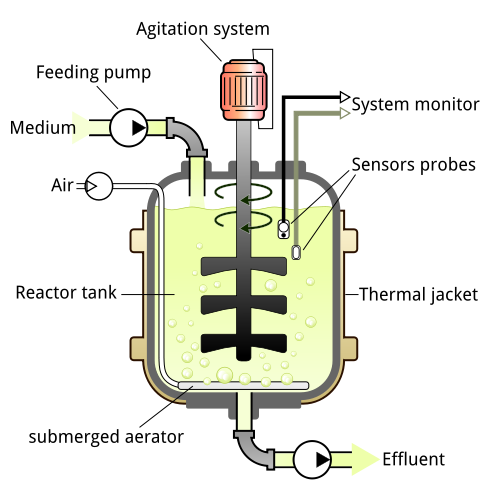
\includegraphics[width=0.7\textwidth]{images/reactor.png}
\caption{Bioreactor.}
\label{fig:split}
\end{figure}
\section{UASB reactor}
An efficient anaerobic digestion (AD) of organic matter is a result of a complex microbial interaction inside a bioreactor. For the high-rate anaerobic digestion of a feedstock, an up flow anaerobic sludge blanket reactor (UASB) is a common choice. 

UASB uses an anaerobic process whilst forming a blanket of granular sludge which suspends in the tank. Wastewater flows upwards through the blanket and is processed (degraded) by the anaerobic microorganisms. The upward flow combined with the settling action of gravity suspends the blanket with the aid of flocculates. The blanket begins to reach maturity at around three months. Small sludge granules begin to form whose surface area is covered in aggregations of bacteria. In the absence of any support matrix, the flow conditions create a selective environment in which only those microorganisms capable of attaching to each other survive and proliferate. Eventually the aggregates form into dense compact biofilms referred to as "granules".Biogas with a high concentration of methane is produced as a by-product, and this may be captured and used as an energy source, to generate electricity for export and to cover its own running power.

\begin{figure}[htbp]
\centering
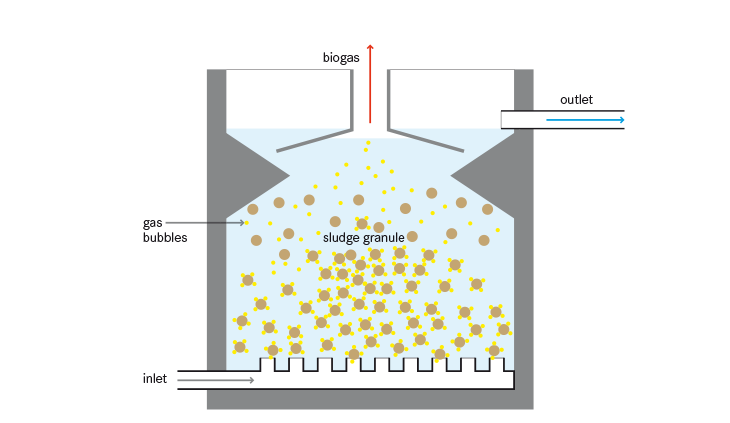
\includegraphics[width=1.0\textwidth]{images/usab.png}
\caption{A USAB reactor.}
\label{fig:usab reactor}
\end{figure}

\section{Background}

The predominant execution of this reactor is because of the specific association of microorganisms into circular granular structures. The process of granulation was first noticed and documented in the early 1980s[citation] and since then many anaerobic granulation theories have been presented. The main reasoning for the granulation per se is the up-flow velocity inside sludge bed of a UASB reactor. Microbial cells moving up with the flow of the feed tend to stick to the other microbial cells. Such sticking behavior prevents a washout of the microbial inoculum from a reactor since the outlet for the digested feed is in the top of the reactor [3,4]. The most widely accepted theory states that granulation starts with a formation of a future granules core, comprised of filamentous methanogenic bacteria Methanothrix, together with Methanosarcina, which secrete extracellular polymers (ECP) [citation]. The surface of this change and become attractive for the oppositely charged anaerobic bacteria that are present in the dispersed inoculum of a UASB[citation]. Chemo-attractancy of other bacteria towards ECPs and substrate around the granule core may also play a major role in the further aggregation and formation of mature granules [citation]. Despite these possible explanations of the granulation process, there is still no agreement on which of the possible theories correctly explain this most important and crucial role of granulation. The key factors of granulation are still to be determined, whether they are physical, biochemical or a combination of physicochemical properties of the cells and the way the organic matter transforms over space and time.

Bioaugmentation is a typical procedure in the field of wastewater treatment, utilized to acquaint another metabolic capacity with either oxygen consuming or anaerobic granules. In this study, we have created a simulation model which is concerned about digesting celloboise, as a major component of microalgae in a bioreactor. Once a mature granule is formed, protein lipid is used as an alternative substrate that will be supplied to a mature granule. Protein, being a main component of cyanobacteria, will promote growth and incorporation of a cell type that can degrade protein (selective pressure). 

Some exploration additionally proposes a requirement for a tight biochemical collaboration to happen between the bioaugmented strain and the available intact community (Citation). Such biochemical interaction together with substrate niche availability will lead to a stratification or compartmentalization of the bioaugmented strain in the granule. Intending to reveal insight to the systems of the anaerobic granulation, current group of metabolic and biochemical cooperations amid bioaugmentation of anaerobic granules can be connected to build up a prescient demonstrate for the bioaugmented granule. A model that can outwardly illustrate shifting stratifications of various trophic microbial gatherings will be of assistance for the designers and scientists, who are working both research center and modern scale anaerobic digesters and wish to improve reactor execution. In the past work, a model of anaerobic granulation was effectively manufactured, and a search engine was utilized to locate the ideal methane generation from the glucose concentration of COD corresponding to the low-strength wastewaters (Doloman et al., 2017). 

\section{Current biological model}

The new model reported here builds up on the basic principles of de novo anaerobic granulation reported earlier and a more complex model is suggested. Described granule formation is based on the aerobic decomposition of cellulose, thus describing a more vigorous microbial network of 5-6 different bacteria. To simulate bioaugmentation process as in the lab anaerobic digesters, new additional bacterial species are introduced to the mature complex granule, together with a specific substrate that can only be decomposed by the new introduced bacterium. Cellulose, being a main carbohydrate component of all plant and algal biomass, was chosen as a substrate of interest due to its relatively complex anaerobic digestion scheme, allowing multiple trophic groups to occupy the same layer in the granule. Lipid derivative was chosen as a substrate of interest that would be degraded with the simulated bioaugmented granule. This derivative, oleate is usually produced as an intermediate from anaerobic degradation of lipids, by glycerol-fermenting acidogenic bacteria (Angleidaki, 1988). Oleate is introduced into the model together with an arbitrary oleate degrading bacterium, providing a full contrast to the decomposition of the cellulose substrate and thus bioaugmenting the granule with the new or additional metabolic capability. Thus, the purpose of this study was to model different scenarios of bioaugmenting anaerobic granule with the novel microbial species: with and without pressure of the available specific substrate.

\begin{figure}[htbp]
\centering
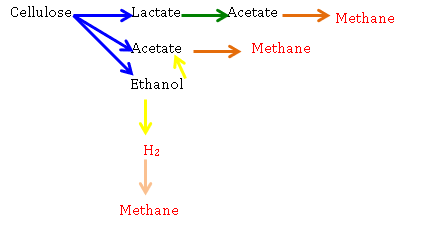
\includegraphics[width=0.7\textwidth]{images/schema1.png}
\caption{Schema of complex granule formation.}
\label{fig:Schema of complex granule formation}
\end{figure}

Current study explores different scenarios of bioaugmenting anaerobic granules with the novel microbial species: with and without pressure of the available specific substrate. The general aim of the study is to expand the knowledge on both successful bioaugmentation experiments and inspire for industrial-scale modifications in anaerobic digestion processes. 

% Please add the following required packages to your document preamble:
% \usepackage[table,xcdraw]{xcolor}
% If you use beamer only pass "xcolor=table" option, i.e. \documentclass[xcolor=table]{beamer}
\begin{table}
\centering
\caption{Microbe responsible for the conversion pathway}
\label{table1}
\begin{tabular}{|l|l|}
\hline
Conversion pathway                                       & Type of microbe responsible \\ \hline
{\color[HTML]{00009B} \textbf{------------\textgreater}} & Clostridium I               \\ \hline
{\color[HTML]{32CB00} \textbf{------------\textgreater}} & Clostridium II              \\ \hline
{\color[HTML]{036400} \textbf{------------\textgreater}} & Methanogen I                \\ \hline
{\color[HTML]{FFC702} \textbf{------------\textgreater}} & Desulfovibrio               \\ \hline
{\color[HTML]{38FFF8} \textbf{------------\textgreater}} & Methanogen II               \\ \hline
{\color[HTML]{FE0000} \textbf{------------\textgreater}} & OleateDegrader              \\ \hline
\end{tabular}
\end{table}



    %
%  This is an example of how a LaTeX thesis should be formatted.  This
%  document contains chapter 2 of the thesis.
%
%  Time-stamp: "[sample-chapter2.tex] last modified by Scott Budge (scott) on 2016-07-28 (Thursday, 28 July 2016) at 08:40:50 on goga.ece.usu.edu"
%
%  Info: $Id: sample-chapter2.tex 967 2016-07-28 15:33:29Z scott $   USU
%  Revision: $Rev: 967 $
% $LastChangedDate: 2016-07-28 09:33:29 -0600 (Thu, 28 Jul 2016) $
% $LastChangedBy: scott $
%

\chapter{MODEL AND EXPERIMENT}

The process of granulation is modeled at two spatial scales in the simulation. At the macro scale, the reactor process is simulated where the cells are introduced into an agitated system (due to the up ow velocity in UASB reactor), cells interact and form multiple agglomerates (centers of granulation). At the mesoscale, simulations are performed that focus on the growth and development of one such agglomerate into a mature granule.

In the macro scale, randomly distributed methanogenic cells (further referred to as “methanogens"), Desulfovibrio and clostridium are introduced into random positions within the reactor. The particles experience mechanical forces due to agitation in the system as well as biomechanical forces due to homogeneous and heterogeneous adhesion and formation of EPS-driven interactions. As a cumulative effect of these forces, cells come close to each other and form several agglomerates.
To closely monitor the growth patterns in the formation of a granule, the mesoscale simulation is designed to focus on the development of a single granule (from the initial agglomerate of all the species particles formed during the macro studies). In UASB bioreactors, granules move freely in an agitated system, where the supplied solutes are relatively mixed. To simulate such a mixed environment for the granule growth, we provide a continuous supply of one solute (Cellobiose) from all the sides of the simulation domain with diffusivity as defined in Table 2.1. The model executes growth reactions that represent the consumption of the supplied glucose by the Clostridium1, which secretes acetate, lactate and ethanol and the consumption of acetate by methanogen, which is converted into the methane gas. The other by solutes produced i.e, lactate and ethanol are consumed by clostridium II and Desulfovibrio respectively to produce acetate and hydrogen respectively. Hydrogen present in the system is consumed by methanogen2 cells to produce methane and acetate produced by clostridium II cells is consumed by methanogen I cells to produce methane as the final product. These reactions and food chains continue to progress for 1500 hours in the simulation and form a mature granule with radius of 630 micro meters as shown in Fig~\ref{fig:granule}.

\begin{figure}[htbp]
\centering
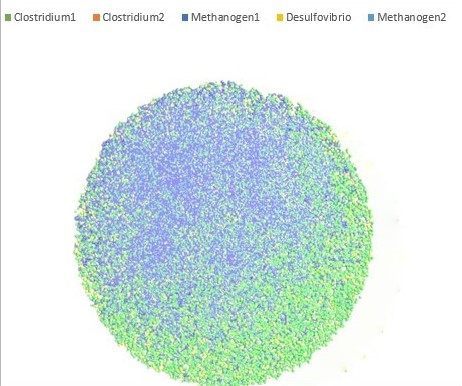
\includegraphics[width=1.0\textwidth]{images/granule.jpg}
\caption{A mature complex granule at the end of 1500 hours.}
\label{fig:granule}
\end{figure}

 
\section{Formation of a complex granule on cellulose}

This simulation is referred to by the name part 1 in the rest of the study.A granule with five types of bacteria (clostridium1, clostridium2, desulfovibrio and two types of methanogens) was formed on the constantly supplied cellobiose, substrate for the clostridium1. All the solutes were formed from the initial conversion of cellobiose into lactate, acetate and ethanol (\ref{fig:Schema of complex granule formation}) . Complex granule was formed after 1000 hrs of computer simulation (corresponding to the 42 days in the lab-scale reactor) and no firm stratification was observed (\textbf{Figure 2 - table with granules and solutes for comparison}), contrary to the previous simulation of granule-fed granule \cite{Doloman et al., 2017} and similar published laboratory studies. Instead, formed granule on the cellobiose resembled a mixed microbial structure, since there was no sharp diffusion gradient of the formed/consumed solutes. Such structure looks similar to the reported laboratory-studied granules fed with complex brewery, cellulose or protein-rich substrate \cite{batstone2004influence, diaz2006phenotypic, baloch2008structural}. Since all three initial cellobiose-digestives (acetate, ethanol and lactate) were produced simultaneously, all three corresponding bacterial consumers (clostridium 2, desulfovibrio and methanogen1) are present in the outer core of the granule, as well as equally distributed throughout the granule depth. The only two bacterial groups that are located closer to the center of the granule are two methanogen types: both acetate and hydrogen utilized by them are the last terminal solutes in the conversion chain of cellobiose. 

After 980 hrs of simulation, there was no death observed in the granule, contrary to the digestion of the glucose fed granule (death occurred within 350 hrs). The dead biomass on cellobiose starts to appear around hour 985 (41 days), and is represented by the ethanol-consuming Desulfovibrios. Around hour 1160 (48days) Clostridium1, consuming cellobiose and those that are located closer to the core of the granule, also start to die, due to the lack of cellobiose in the core of the granule caused by the diffusion limitation. 

\section{Bioaugmentation with lipid-degrading bacteria}

To investigate the possibility of incorporating a new bacterium type into the cellobiose-fed granule, a lipid-degrading bacteria was chosen. Both scenarios with or without substrate pressure were investigated.

\subsection{Incorporation of lipid-degrading bacteria with oleate as a sole substrate}

This simulation is referred to by the name part 2.1 in the rest of the study.When lipid derivative, oleate, was used as a sole feed for the established granule on cellobiose, OleateDegraders were successfully incorporated into the granule, residing mainly in the outer layer of the granule (Figure 2, video with species count). Even though early OleateDegraders did distribute randomly in the granule (until around 450 hrs), they are steadily pushed to the outer layers of the granule, potentially due to the presence there of higher oleate quantities. A sharp oleate gradient cannot be visually detected on the oleate video, due to the still low numbers of the incorporated OleateDegraders. Nevertheless, those few successfully incorporated OleateDegraders are highly active in the granule, since there is a constant decrease in the total amount of the oleate in the system and an increase in the amount of produced acetate over time (REFERENCE GRAPHS OF TOTAL SOLUTES AND VIDEOS). Note that acetate is produced exactly at the locations of the newly incorporated OleateDegraders.

A peculiar architecture can be seen with the "pockets" of methanogenic bacteria randomly distributed around the granule. This is caused by the sudden death of other bacteria (clostridium1,2, desulfovibrio) as soon as the residual substrates are depleted from initial growth on cellobiose (Part 1), since in this 2.1 simulation oleate is the only supplied feed for the granular growth. By judging the distribution of the methanogenic "pockets" one can predict where the food (acetate) was supplied to them by clostridium1 and desulfovibrios. The result of the sudden death of the acetate-supplying bacteria is an irregular pattern of methanogens distribution across the whole granule, both in density and number. Similar "pocketing" behavior of other acetoclastic methanogenic bacteria in anaerobic granule were reported by \cite{schmidt1999immobilization}. 

Current modeling platform doesn't have an algorithm for a "shrinking" and eliminating of the dead particles, as division of granules and their further growth into "daughter" smaller granules is beyond the scope of the current work. However, one can theoretically predict a division of the initial cellobiose-fed granule into the multitude of the new "daughter" granules with only two bacterial species: Methanogen1 and OleateDegraders. The number of big blue Methanogen1 clusters as seen in the granule image(\ref{fig:part2.1}) possibly can be equal to the number of the new small granules to be formed due to the bioaugmentation with OleateDegraders. Nevertheless, this "daughter" division might not take place in the anaerobic reactor, if the applied sheer stress of the up-flow velocity in the UASB reactors is not high enough to physically break the granule with dead particles in it. In this case newly augmented granules will continue to grow with so-called cavities, as described in laboratory studies. 

\subsection{Incorporation of lipid-degrading bacteria with both cellulose and oleate as substrates}

This simulation is referred to by the name part 2.2 in the rest of the study.Contrary to the previous study where oleate was the sole supplied substrate for the granular growth, this experiment investigated a lack of substrate-pressure on the success of the bioaugmentation with OleateDegraders.

The OleateDegraders are incorporated into the outer layer of the granule (Supplementary material Video of 2.2 part) and are successfully present there till 720 hrs (30 days) of the simulation. After this, OleateDegraders are sloughed from the granule's outer layer and washed out.Thus, availability of the proper substrate niche in the granule does not necessarily leads to the successful incorporation of the new species. If the granule is supplied with the old type of feed that can sustain viability of the complete bacterial population inside, chances of the new species to be incorporated into a mature and rapidly developing consortia are very low.  

\section{Bioaugmentation with ethanol-degrading bacteria}

Another question that was necessary to study is: Can one bioaugment with bacteria that is needed for the middle step of the digestion? On the contrary to introducing both new substrate and a bacteria, in this part we investigate addition of a bacterium that is critical for some steps of the originally present cellobiose bioconversion scheme, ethanol degrader and a hydrogen producer: desulfovibrio (fig:\ref{fig:Schema of complex granule formation}).

\subsection{Incorporation of ethanol-degrading bacteria after initial granulation}

This simulation is referred to by the name part 2.3 in the rest of the study.To explore how incorporation of desulfovibrios into the mature granule changes the solutes profile and granular architecture, we first simulated development of the initial granule without desulfovibrio (REFERENCE VIDEO 3.1.1). One can note a poor microbial diversity in the granule and a 20-fold decrease in the averaged produced methane amount. In the next stage, desulfovibrios were introduced back to the granule and cells were successfully incorporated, rapidly filling the whole depth of the granule and consuming the accumulated ethanol. One can also note that despite the fact that hydrogen was intensely produced by the desulfovibrios, it was not converted into the methane  (\ref{fig:Schema of complex granule formation}). This is because all the methanogens2 were already dead by the time incorporation of desulfovibrios took place. This finding has an important practical application, since it addresses the speed which should be used if bioaugmentation is planned. Bacteria tend to die, if not forming dormant spores, and this can break an important metabolic chain and cause significant fluctuations in pH and even shifts the total product yield (needless to say that in real digester shifts to high amounts of hydrogen would crash the whole system and prohibit aceticlastic methane-producing activity. 

\subsection{Re-supply of ethanol-degrading bacteria to the established consortia}

This simulation is referred to by the name part 2.4 in the rest of the study.Sometimes bioaugmentation fails if there is no substrate niche available for the newly-introduced microbe to occupy. Or, if there is a local bacteria in the granule that is already performing the metabolic function of interest for the bioaugmentation. In this case, competition for the same type of substrate and a place in a constantly growing granule may lead to unsuccessful bioaugmentation. To study this scenario, we introduced additional ethanol-consuming and hydrogen-producing bacteria (desulfovibrio2) into a well-formed and maintained granule (taken from the Part 1 simulation with a complete metabolic pathway).   

The results demonstrate that additional ethanol-consuming bacteria (desulfovibrio2) were rapidly incorporated to the mature granule with its own population of desulfovibrio1. However, newly introduced bacteria quickly die off after 144 hours of simulation: possibly due to both slaughing of the biomass above 630 $\mu$m limit and due to the competition for the ethanol with originally present desulfovibrio1. One can note a very scarce amount of ethanol of the solute graphs at the end of the simulation (MAIN TABLE-FIGURE) and throughout the 1000 hour simulation (part 2.4 VIDEO IN THE SUPPLEMENTAL MATERIAL).


\begin{table}
\centering
\caption {Parameters used in model and their correspondent values}
\smallskip


	\def\arraystretch{1.1}%
	\setlength{\tabcolsep}{1em}
	\begin{tabular}{|p{6cm}|p{1.2cm}|p{1.4cm}|p{1.5cm}|p{3cm}|}
		\hline
		\multicolumn{5}{|c|}{	\textbf{Parameter Summary}} \\
		\hline
		\textbf{Model parameter   }  &	\textbf{Symbol } 	&	\textbf{ Value }& 	\textbf{Unit}& 	\textbf{References}\\
		\hline
		\multicolumn{5}{|c|}{	\textbf{Solutes}} \\
		\hline
		Diffusion of Cellobiose in liquid  &$ D_{C}	$    & 5.1x$10^{-6}$ &$m^{2}$ /day& \cite{}  \\ \cline{1-5}	
		Diffusion of Oleate in liquid	 &$ D_{O} $	& 2.85x$10^{-5}$ &$m^{2}$ /day&\cite{} \\ \cline{1-5}
		Diffusion of Lactate in liquid	 &$ D_{L} $	& 9.07x$10^{-5}$ &$m^{2}$ /day&\cite{} \\ \cline{1-5}
        Diffusion of Acetate in liquid	 &$ D_{A} $	& 1.05x$10^{-4}$ &$m^{2}$ /day&\cite{} \\ \cline{1-5}
        Diffusion of Ethanol in liquid	 &$ D_{E} $	& 7.25x$10^{-5}$ &$m^{2}$ /day&\cite{} \\ \cline{1-5}
        Diffusion of Hydrogen in liquid	 &$ D_{H} $	& 3.89x$10^{-4}$ &$m^{2}$ /day&\cite{} \\ \cline{1-5}
		Diffusion of Methane in liquid  & $D_{M}	$	& 1.29x$10^{-4}$ &$m^{2}$ /day& \cite{haynes2012CRC}\\  \cline{1-5}
		Biofilm Diffusivity  & $ \gamma	$	&	30 & \% & \cite{lens2003diffusional}\\ \cline{1-5}
		
		\multicolumn{5}{|c|}{\textbf{Clostridium I:}} \\
		\cline{1-5}
		Cell mass   & $ B_{c1}$&	500 & fg& \cite{kubitschek1990cell} \\ \cline{1-5}
		Division radius  & 	&2&$\mu$m &\cite{sowers1984methanosarcina}\\ \cline{1-5}
		Maximum growth rate	& $\hat{\mu_{c1}}$ & 0.15& $h^{-1}$&\cite{kubitschek1990cell}, \cite{gavala2003kinetics, ibba1991two} \\ \cline{1-5}
		Substrate saturation constant& $ Ks_{C} $ &	2.5&g/L&\cite{kalyuzhnyi1997batch, ibba1991two}  \\ \cline{1-5}
		Biomass conversion rate& $ \alpha_{bc}$	&0.203& $\frac{g_{biomass}}{g_{cellobiose}}$&\cite{ibba1991two, bhunia2008analysis}  \\ \cline{1-5}
		Substrate conversion rate&$ \alpha_{ac}$&	0.45& $\frac{g_{acetate}}{g_{cellobiose}}$&\cite{gavala2003kinetics, ibba1991two}  \\ \cline{1-5}
        Substrate conversion rate&$ \alpha_{lc}$&	0.0096& $\frac{g_{lactate}}{g_{cellobiose}}$&\cite{gavala2003kinetics, ibba1991two}  \\ \cline{1-5}
        Substrate conversion rate&$ \alpha_{ec}$&	0.28& $\frac{g_{ethanol}}{g_{cellobiose}}$&\cite{gavala2003kinetics, ibba1991two}  \\ \cline{1-5}
		Death delay&	&48 & $h$& estimated\\ \cline{1-5}
		Death threshold&	&0.02 & g/L& estimated\\ \cline{1-5}
        
        \multicolumn{5}{|c|}{\textbf{OleateDegrader ????Check mass, radius and Dying switches:}} \\
		\cline{1-5}
		Cell mass   & $ B_{o}$&	500 & fg& \cite{kubitschek1990cell} \\ \cline{1-5}
        Division radius  & 	&2&$\mu$m &\cite{}\\ \cline{1-5}
		Maximum growth rate	& $\hat{\mu_{o}}$ & 0.02& $h^{-1}$&\cite{} \\ \cline{1-5}
		Substrate saturation constant& $ Ks_{O} $ &	0.02&g/L&\cite{}  \\ \cline{1-5}
        Product inhibition constant& $ Ki_{Ap} $ &	5&g/L&\cite{}  \\ \cline{1-5}
        Biomass conversion rate& $ \alpha_{bo}$	&0.1& $\frac{g_{biomass}}{g_{oleate}}$&\cite{}  \\ \cline{1-5}
		Substrate conversion rate&$ \alpha_{ao}$&	1.85& $\frac{g_{acetate}}{g_{ethanol}}$&\cite{}  \\ \cline{1-5}
        Death delay&	&96 & $h$& estimated\\ \cline{1-5}
		Death threshold&	&0.00001 & g/L& estimated\\ \cline{1-5}
        
        \multicolumn{5}{|c|}{\textbf{Clostridium II:}} \\
		\cline{1-5}
		Cell mass   & $ B_{c2}$&	500 & fg& \cite{kubitschek1990cell} \\ \cline{1-5}
		Division radius  & 	&2&$\mu$m &\cite{}\\ \cline{1-5}
		Maximum growth rate	& $\hat{\mu_{c2}}$ & 0.144& $h^{-1}$&\cite{}, \cite{} \\ \cline{1-5}
		Substrate saturation constant& $ Ks_{L} $ &	0.03&g/L&\cite{}  \\ \cline{1-5}
		Biomass conversion rate& $ \alpha_{bc2}$	&0.06& $\frac{g_{biomass}}{g_{lactate}}$&\cite{}  \\ \cline{1-5}
		Substrate conversion rate&$ \alpha_{al}$&	0.45& $\frac{g_{acetate}}{g_{lactate}}$&\cite{}  \\ \cline{1-5}
        Death delay&	&118 & $h$& estimated\\ \cline{1-5}
		Death threshold&	&0.00001 & g/L& estimated\\ \cline{1-5}
        	\end{tabular}
	\label{parametersTable}
\end{table}


\begin{table}
\caption{ Parameters used in model and their correspondent values}
\smallskip
	
	
	\def\arraystretch{1.0}%
	\setlength{\tabcolsep}{1em}
	\begin{tabular}{|p{5cm}|p{1.2 cm}|p{1.2cm}|p{1.2cm}|p{3cm}|}
		\hline
		\multicolumn{5}{|c|}{	\textbf{Parameter Summary}} \\
		\hline
		\textbf{Model parameter   } & \textbf{Symbol } 	&	\textbf{ Value }& 	\textbf{Unit}& 	\textbf{References}\\
		\hline

        \multicolumn{5}{|c|}{\textbf{Desulfovibrio:}} \\
		\cline{1-5}
		Cell mass   & $ B_{d}$&	500 & fg& \cite{kubitschek1990cell} \\ \cline{1-5}
        Mass of EPS capsule   & &	10&fg&\cite{}\\ \cline{1-5}
		Division radius  & 	&2&$\mu$m &\cite{}\\ \cline{1-5}
		Maximum growth rate	& $\hat{\mu_{d}}$ & 0.125& $h^{-1}$&\cite{} \\ \cline{1-5}
		Substrate saturation constant& $ Ks_{E} $ &	4.5x$10^{-4}$&g/L&\cite{}  \\ \cline{1-5}
        Product inhibition constant& $ Ks_{A} $ &	7.2&g/L&\cite{}  \\ \cline{1-5}
        Substrate inhibition constant& $ Ki_{E} $ &	80.5&g/L&\cite{}  \\ \cline{1-5}
		Biomass conversion rate& $ \alpha_{be}$	&0.22& $\frac{g_{biomass}}{g_{ethanol}}$&\cite{}  \\ \cline{1-5}
		Substrate conversion rate&$ \alpha_{ac}$&	1.3& $\frac{g_{acetate}}{g_{ethanol}}$&\cite{}  \\ \cline{1-5}
        Substrate conversion rate&$ \alpha_{hc}$&	0.17& $\frac{g_{hydrogen}}{g_{ethanol}}$&\cite{}  \\ \cline{1-5}
        Death delay&	&96 & $h$& estimated\\ \cline{1-5}
		Death threshold&	&0.00001 & g/L& estimated\\ \cline{1-5}
		
		\multicolumn{5}{|c|}{\textbf{Methanogens I:}} \\
		\cline{1-5}
		Cell mass 	 & $ B_{m1} $&1000 &fg&\cite{sowers1984methanosarcina}\\ \cline{1-5}
		Mass of EPS capsule   & &	10&fg&\cite{moletta1986dynamic}\\ \cline{1-5}
		Division radius  & 	&2&$\mu$m &\cite{sowers1984methanosarcina}\\ \cline{1-5}
		Maximum growth rate& $\hat{\mu_{m1}}$&	0.029&  $h^{-1}$&\cite{moletta1986dynamic, nishio1990methanogenesis}\\ \cline{1-5}
		Substrate saturation constant& $ Ks_{Ac} $&	1.02& g/L&\cite{moletta1986dynamic}\\ \cline{1-5}
        Substrate inhibition constant& $ Ki_{Ac} $ &	48.64&g/L&\cite{gavala2003kinetics, ibba1991two}  \\ \cline{1-5}
		Biomass conversion rate&$ \alpha_{ba}$&	0.15&$ \frac{g_{biomass}}{g_{acetate}}$ &\cite{nishio1990methanogenesis, kalyuzhnyi1997batch}\\ \cline{1-5}
		Substrate conversion rate&$ \alpha_{ma}$	&0.26 & $\frac{g_{methane}}{g_{acetate}}$&\cite{nishio1990methanogenesis}\\ \cline{1-5}
		Death delay&	&48 & $h$&estimated\\ \cline{1-5}
		Death threshold&	&0.00001 & g/L&estimated\\ \cline{1-5}
        
		\multicolumn{5}{|c|}{\textbf{Methanogens II:}} \\
		\cline{1-5}
		Cell mass 	 & $ B_{m2} $&1000 &fg&\cite{sowers1984methanosarcina}\\ \cline{1-5}
		Mass of EPS capsule   & &	10&fg&\cite{moletta1986dynamic}\\ \cline{1-5}
		Division radius  & 	&3&$\mu$m &\cite{sowers1984methanosarcina}\\ \cline{1-5}
		Maximum growth rate& $\hat{\mu_{m2}}$&	0.02&  $h^{-1}$&\cite{moletta1986dynamic, nishio1990methanogenesis}\\ \cline{1-5}
		Substrate saturation constant& $ Ks_{H} $& 18x$10^{-6}$& g/L&\cite{moletta1986dynamic}\\ \cline{1-5}
        Biomass conversion rate&$ \alpha_{bh}$&	0.033&$ \frac{g_{biomass}}{g_{hydrogen}}$ &\cite{nishio1990methanogenesis, kalyuzhnyi1997batch}\\ \cline{1-5}
		Substrate conversion rate&$ \alpha_{mh}$	&0.26 & $\frac{g_{methane}}{g_{hydrogen}}$&\cite{nishio1990methanogenesis}\\ \cline{1-5}
		Death delay&	&48 & $h$&estimated\\ \cline{1-5}
		Death threshold&	&0.000001 & g/L&estimated\\ \cline{1-5}
		
	
	\end{tabular}
	\label{parametersTable}
\end{table}

Seven solutes: cellobiose ($S_{C}$), oleate ($S_{O}$), lactate ($S_{L}$), acetate ($S_{A}$), ethanol ($S_{E}$), hydrogen ($S_{H}$), and methane ($S_{M}$) exist within the reactor model. The distribution of these solutes is controlled by Equations~\ref{s1}, \ref{s2}, \ref{s3}, \ref{s4}, \ref{s5}, \ref{s6}, and \ref{s7}, respectively. The diffusion coefficients and reaction rates take different forms for each region depending upon the spatial distribution of six types of biomass: clostridium1 (generic bacterium degrading cellobiose) ($B_c1$), clostridium2 (generic bacterium degrading lactate) ($B_c2$), oleateDegraders ($B_o$), desulfovibrio (generic bacterium degrading ethanol) ($B_d$), and two types of methanogens ($B_m1$), ($B_m2$), degrading acetate and hydrgen respectively. These relationships are described in the Equation~\ref{s8}. 
The effective diffusion coefficient is decreased within the granule compared with the liquid value in order to account for the increased mass transfer resistance. The diffusivity values used for the model (specified in  Table 1) are taken from literature related to biofilm diffusivity studies \cite{stewart2003diffusion,lens2003diffusional}.


\begin{equation}
\frac{\partial S_{C}}{\partial t} = B(x,y).D_{C}.\frac{\bigtriangledown^{2} S_{C}}{{\partial x}{\partial y}}- \mu_{c1}(S_{C},S_{A}).\frac{B_{c1}}{\alpha_{bc1}}
\label{s1}
\end{equation}

\begin{equation}
\frac{\partial S_{O}}{\partial t} = B(x,y).D_{O}.\frac{\bigtriangledown^{2} S_{O}}{{\partial x}{\partial y}}- \mu_{o}(S_{O},S_{A}).\frac{B_{o}}{\alpha_{bo}}
\label{s2}
\end{equation}

\begin{equation}
\frac{\partial S_{L}}{\partial t} = B(x,y).D_{L}.\frac{\bigtriangledown^{2} S_{L}}{{\partial x}{\partial y}}+ \mu_{c1}(S_{C}).\frac{B_{c1}}{\alpha_{bc1}}
\label{s3}
\end{equation}

\begin{equation}
\frac{\partial S_{A}}{\partial t} = B(x,y).D_{A}.\frac{\bigtriangledown^{2} S_{A}}{{\partial x}{\partial y}}+ \mu_{d}(S_{E},S_{A}).\frac{B_{d}}{\alpha_{bd}}+ \mu_{c2}(S_{L}).\frac{B_{c2}}{\alpha_{bc2}}
\label{s4}
\end{equation}

\begin{equation}
\frac{\partial S_{E}}{\partial t} = B(x,y).D_{E}.\frac{\bigtriangledown^{2} S_{E}}{{\partial x}{\partial y}}+ \mu_{c1}(S_{C}).\frac{B_{c1}}{\alpha_{bc1}}
\label{s5}
\end{equation}

\begin{equation}
\frac{\partial S_{H}}{\partial t} = B(x,y).D_{H}.\frac{\bigtriangledown^{2} S_{H}}{{\partial x}{\partial y}}+ \mu_{d}(S_{E},S_{A}).\frac{B_{d}}{\alpha_{bd}}
\label{s6}
\end{equation}

\begin{equation}
\frac{\partial S_{M}}{\partial t} = B(x,y).D_{M}.\frac{\bigtriangledown^{2} S_{M}}{{\partial x}{\partial y}}+ \mu_{m1}(S_{A}).\frac{B_{m1}}{\alpha_{bm1}}+ \mu_{m2}(S_{H}).\frac{B_{m2}}{\alpha_{bm2}}
\label{s7}
\end{equation}

where,

\begin{equation}
B(x,y)=\left\{
\begin{array}{ll}
\begin{tabular}{cc}

1.0    & if location $x,y$ contains no biomass\\

$\gamma$ & if location $x,y$ contains biomass
\end{tabular}

\end{array}
\right.
\label{s8}
\end{equation}

Equations \ref{b1}, \ref{b2}, \ref{b3}, \ref{b4}, \ref{b5} and \ref{b6}  describe changes in the biomass of all growing 6 bacterial cell types (clostridium1, clostridium2, oleateDegraders, desulfovibrio and two types of methanogens) as a function of local cellobiose, acetate, lactate, ethanol, methane and hydrogen concentrations. A discrete switching mechanism is used to model cell death due to a lack of food. The switching mechanism is defined as the function $die(B_i)$ in the equations. For example, Clostridium1 cells are converted to dead cells when the amount of cellobiose is below a threshold value (death threshold in Table 1) for a period of 48 hours. Similarly,  the Methanogen1 cells are converted to dead cells when the amount of acetate is below a threshold value (death threshold in Table 1) for a period of 48 hours. The rate of increase in dead cell mass is define in Equation~\ref{b7}. The parameter values for controlling cell death are estimated due to the lack of studies quantifying the response of described cell types to nutritional stress.

\begin{equation}
\frac{\partial B_{c1}}{\partial t} = \mu_{c1}(S_{C}) B_{c1}-die(B_{c1})
\label{b1}
\end{equation}


\begin{equation}
\frac{\partial B_{c2}}{\partial t} = \mu_{c2}.(S_{L}). B_{c2}-die(B_{c2})
\label{b2}
\end{equation}

\begin{equation}
\frac{\partial B_{o}}{\partial t} = \mu_{o}.(S_{O}, S_{A}). B_{o}-die(B_{o})
\label{b3}
\end{equation}

\begin{equation}
\frac{\partial B_{d}}{\partial t} = \mu_{d}.(S_{E}, S_{A}). B_{d}-die(B_{d})
\label{b4}
\end{equation}

\begin{equation}
\frac{\partial B_{m1}}{\partial t} = \mu_{m1}.(S_{A}). B_{m1}-die(B_{m1})
\label{b5}
\end{equation}

\begin{equation}
\frac{\partial B_{m2}}{\partial t} = \mu_{m2}.(S_{H}). B_{m2}-die(B_{m2})
\label{b6}
\end{equation}

\begin{equation}
\frac{\partial B_{dead}}{\partial t} = die(B_{c1}) + die(B_{c2}) + die(B_o) + die(B_d) + die(B_{m1}) + die(B_{m2})
\label{b7}
\end{equation}

The growth rates: of clostridium1 is $\mu_{c1}(S_{C})$, defined in Equation~\ref{cellobiosedegradation}, the growth rate of clostrodium2 is $\mu_{c2}(S_{L})$, defined in Equation~\ref{lactatedegradation}, the growth rate of oleateDegraders is $\mu_{o}(S_{O}, S_{A})$, defined in Equation~\ref{oleatedegradation}, the growth rate of desulfovibrio is $\mu_{d}(S_{E}, S_{A})$, defined in Equation~\ref{ethanoldegradation}, the 
methanogens1 is $\mu_{m1}(S_{A})$ defined in Equation~\ref{acetatedegradation} and the growth rate of methanogen2 is $\mu_{m2}(S_{H})$, defined in Equation~\ref{hydrogendegradation}.
From the equations can be seen that growth of Clostridium1, Clostridium2 and Methanogen2 follows Monod growth kinetic, while growth of OleateDegraders has also product inhibition involved and both equations ~\ref{ethanoldegradation} and ~\ref{acetatedegradation} for Desulfovibrios and Methanogen1 demonstrate Haldane growth kinetic, substrate and product inhibition. The Java code in \textsl{cDynoMiCs} was manipulated to add functionality of describing bacterial growth via Haldane kinetic. 

\begin{equation}
\mu_{c1}(S_{C})={\hat{\mu}_{c1}}\frac{{S_{C}}}{{K_{sC}+S_{C}}}
\label{cellobiosedegradation}
\end{equation}

\begin{equation}
\mu_{c2}(S_{L})={\hat{\mu}_{c2}}\frac{{S_{L}}}{{K_{sL}+S_{L}}}
\label{lactatedegradation}
\end{equation}

\begin{equation}
\mu_{o}(S_{O}, S_{A})=\hat{\mu}_{o}.\frac{{S_{O}}}{{(K_{sO}+S_{o})}}.\frac{K_{i_Ap}}
{{(K_{i_Ap}+S_{A}})}
\label{oleatedegradation}
\end{equation}

\begin{equation}
\mu_{d}(S_{E}, S_{A})=\hat{\mu}_{d}.\frac{{S_{E}}}{{(K_{sE}+S_{E}+\frac{S_{E}^{2}}{K_{ie}})}}.\frac{K_{i_A}}
{{(K_{i_A}+S_{A}})}
\label{ethanoldegradation}
\end{equation}

\begin{equation}
\mu_{m1}(S_{A})=\hat{\mu}_{m1}.\frac{{S_{A}}}{{(K_{sAc}+S_{A}+\frac{S_{A}^{2}}{K_{iAc}})}}
\label{acetatedegradation}
\end{equation}

\begin{equation}
\mu_{m2}(S_{H})={\hat{\mu}_{m2}}\frac{{S_{H}}}{{K_{sH}+S_{H}}}
\label{hydrogendegradation}
\end{equation}

The source code of \textsl{cDynoMiCs} was also modified to introduce a new \textbf{\textit{sloughing}} function, which destroys all the granular biomass that grows above the set granule diameter. Sloughing is needed to simulate a UASB-like environment in the model. Granules in a UASB reactor are constantly under the sheer stress from the continuously flowing feed in the upflow mode. Thus, published works report a certain diameter threshold, above which granule do not grow in the UASB-type reactor. Current study uses a diameter of 630 $\mu$m (this number was mostly picked to decrease computational powers required to compute a bigger granule). The value of the maximum granular diameter is specified in the XML instructions. The \textbf{\textit{sloughing}} function runs for every grid position in the simulation and determines whether a grid location should be slaughtered or not, based on the XML-specified maximum diameter. 

Instructions in the XML also include locations of the new species to be introduced to the already formed granule. When needed, new particles were supplied in the four corners of the square 

Current study reports incorporation of additional bacterial species into the already formed granule. Instructions for additional supply of the species that will be incorporated are provied in the xml file, which can be found for each simulation part in the Github source code page. Briefly, new species are introduced to the simulation environment by specifying their correspondent x,y and z coordinates. In all the simualtions with incorporation of new species, those species were initially provided in the four corners of the 508 $\mu$m $\times$ 508  $\mu$m  (2D) domain. 



\chapter{METHOD}

An agent-based simulator framework, cDynoMiCs [30] is used in this experiment. cDynoMiCs is an extension of iDynomics framework developed by the Kreft group at University of Birmingham specifically for modeling biofilms. cDynoMiCs includes eucaryotic cell modeling processes with the addition of extracellular matrix and cellular mechanisms such as tight junctions and chemotaxis. Each cell is represented as a spherical particle, which has a particular biomass, and implements type and species-specific mechanisms to reproduce cellular physiology. Biochemically, particles can secrete or uptake chemicals that are diffused through the domain by executing reactions. Biomechanically, particles exhibit homogeneous and heterogeneous adhesion, and the formation of tight junctions. Particles model growth by increasing their biomass according to metabolic reactions and split into two particles once a maximum radius threshold is reached. They can also switch from one type of particle to another based on specific microenvironmental conditions and internal states. The simulation process interleaves biomechanical stress relaxation where the particles are moved in response to individual forces, along with the resolution of biochemical processes such as secretion, uptake, and diffusion by a differential equation solver. We assume that the solute fields are in a pseudo steady-state with respect to biomass growth.

Particle growth and division can cause particles to overlap, creating biomechanical stress. To resolve this problem a process called shoving is implemented. When the distance between two particles is less than a fixed threshold set by the particle size, a repulsive force is generated to push them apart, proportional to the overlap distance between the two particles. Then the relaxation process commences that iteratively moves each particle in response to its net force, then recalculates the forces due to the movement. The process terminates when only negligible forces remain, and the system has reached a pseudo steady state.

The typical flow of control and data in the framework is shown in Fig: where amid a solitary worldwide timestep, dynamics of the solute concentration fields, the bulk compartment and the agents are applied independently, in spite of the fact that the progression of each rely upon the present condition of the others (Fig:\ref{fig:algo}). Addressing each class of dynamics separately is possible because they all operate on different timescales (Picioreanu et al., 1999). In addition, the dynamics of the agents are further broken down into smaller timesteps to account for the varied processes affecting agent growth, division and movement, as well as any additional processes an agent may carry out. Once these steps are completed, erosion effects are applied to the biofilm structure as a whole, the global time is incremented, and the next timestep taken.
\begin{figure}[htbp]
\centering
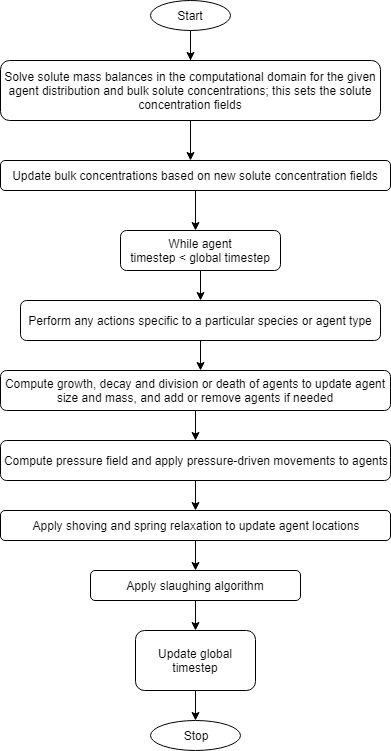
\includegraphics[width=0.7\textwidth]{images/algo.jpg}
\caption{ Pseudo-code describing one global timestep iteration of the individual-based simulator.}
\label{fig:algo}
\end{figure}
cDynoMiCs adds new functionality to the Java code of iDynomics and extends the XML protocol, used to specify many different types of simulations. iDynomics writes plain-text XML files as output, and these may be processed using any number of software tools, such as Matlab,R and python. In addition to XML files, iDynoMiCS also writes files for POV-Ray that is used to render 3-D ray-traced images(Fig:\ref{fig:granule}) of the simulation.

In addition to the cDynoMiCs project, we made following enhancements in the framework to achieve the stated results:

\section{Fixing the Haldane kinetic class to incorporate Haldane reactions}

The Haldane kinetic reaction is responsible for the growth of Desulfovibrio and Methanogen I. Sulfate-reducing bacteria (represented here by Desulfovibrio) are inhibited by both substrate and product – ethanol and acetate. But not hydrogen. The growth reaction is the following (combined both Haldane kinetics and SimpleInhibition), where µmax=maximum growth rate for Desulfovibrio, KSEtOH =saturation constant of ethanol, SEtOH=concentration of ethanol,   = inhibition constant for ethanol, KIAc = inhibition constant for acetate on Desulfovibrio, SAc=concentration of acetate:

The HaldaneKinetic class was lacking some critical functionality which needed to be implemented in order to run the haldane reactions.We added following functions in haldanekinetic class to fix this:

\subsection{Default Constructor to initialize the parameters with kinetic coefficients}

Haldane Kinetic reaction is specified in the XML as shown in Fig:\ref{fig:haldanexml.png} below:

\begin{figure}[htbp]
\centering
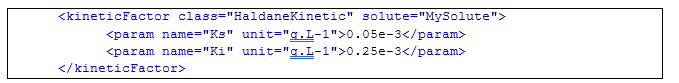
\includegraphics[width=1.0\textwidth]{images/haldanexml.png}
\caption{part of input xml where haldane reaction is defined}
\label{fig:haldanexml}
\end{figure}

Where Ks and Ki are kinetic coefficients for the reaction, to assign these values defined in the XML to the parameters in haldane Kinetic class, the instance variables Ks and Ki are assigned to the respective values using the newly defined constructor.

\subsection{Creating KineticDiff() method to update the growth rate of cells}

We created a new method to implement the math behind the reaction. The method takes 3 parameters, current solute value, coefficient values the parameter table and the index of the grid. It updates the growth rate based on these parameters and equation() and returns the updated value.

\section{Implementing a new sloughing algorithm}

To consider the agitation caused inside the bioreactor due to the up-flow velocity and other factors, we need to create and implement an algorithm which slaugh every cell which is beyond a predefined maximum radius value from the center of the granule. We created an algorithm which reads two values from the XML:

\begin{itemize}
\item The maximum radius of the granule defined under “Agent grid” section in the XML by the parameter name ‘\textbf{MaximumGranuleRadius}’.
\item The value of ‘\textbf{sloughDetachedBiomass}’ parameter defined under “Agent grid” section in the XML which is used to turn the sloughing algorithm on or off.
\end{itemize}
These parameters help us to add new functionality in the project without altering the current methods or code.

The algorithm described by Fig:\ref{fig:sloughingalgo} runs for every grid position and determines whether a grid location should be eligible for  sloughing or not.

\begin{figure}[htbp]
\centering
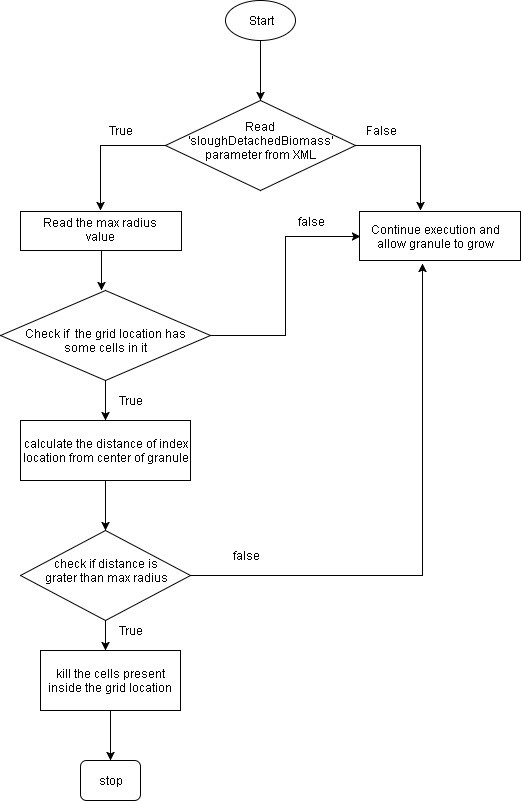
\includegraphics[width=1.0\textwidth]{images/sloughingalgo.jpg}
\caption{Algorithm for sloughing.}
\label{fig:sloughingalgo}
\end{figure}
\section{Transferring species from one simulation to another}

To perform biogmentation, we needed to place the granule into a different bulk which contains some other solutes and while we transfer the granule to the new bulk environment,  all the species cells should stay together in the same position as they were in the last stage of initial simulation. To achieve this, we implemented a new functionality that enables us to copy the contents of last generated agent State file from a simulation and initialize the species distribution of new simulation using the contents of that file so that we would have all the species cells in the same count and locations in the new simulation.We can enable or disable this feature from the xml itself by setting the the value of parameter 'useAgentFile' to true or false so that the existing functionalities won't be altered.

While initializing the agent grid with the species cells in the very first stage of a simulation, we check for the value of the 'useAgentFile' parameter in input xml and if it is set to true, we call a function that initializes the grid positions using the values of the last generated Agent state file of the parent simulation.  

\section{Transferring solutes from one simulation to another}

In some cases of biogmentation, it is also required to copy the solutes present in one simulation to another along with the whole granule in order to closely match the previous bulk environment along with addition of other solutes in the new simulation.To achieve this, we implemented a new functionality that enables us to copy the contents of last generated env State file from a simulation and initialize the solute distribution new simulation using the contents of that file so that we would have all the solutes in the same amount and locations in the new simulation.We can enable or disable this feature from the xml itself by setting the value of parameter 'useSoluteFile' to true or false so that the existing functionalities won't be altered.

While initializing the agent grid with the solute concentrations in the very first stage of a simulation, we check for the value of the 'useSoluteFile' parameter in input xml and if it is set to true, we call a function that initializes the solutes in the grid using the values of the last generated Env state file of the parent simulation.  

\section{Miscellaneous scripts for result analysis}

While the simulation produces a large amount of data files in XML format, we need to get meaningful insights from this data and to achieve this, we generated various graphs and images which accurately describes the granule formation and biogmentation process. 

\subsection{Heatmap for visualizing solute concentrations(MATLAB)}

To better understand the distribution of the solutes in the grid, we used solute concentration files of each solute that are generated after every iteration as inputs to the matlab scripts which generates detailed heatmap images for each solute.This matlab script runs iteratively for each solute type and saves the heatmap images (Fig:\ref{fig:heatmap})in a local folder.


\begin{figure}[htbp]
\centering
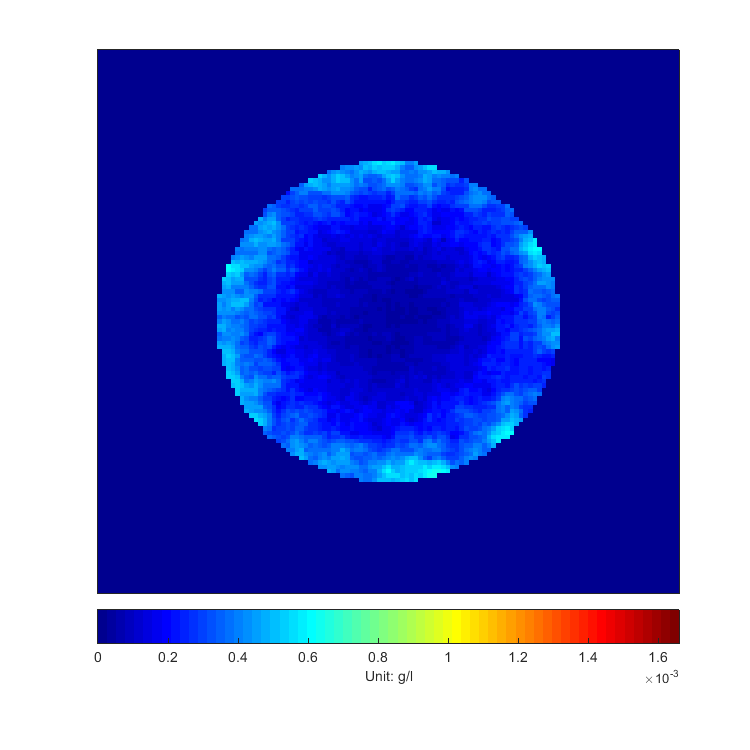
\includegraphics[width=0.6\textwidth]{images/Ethanol_solute_640.png}
\caption{A heatmap representing distribution of solute }
\label{fig:heatmap}
\end{figure}


\subsection{Spatial distribution analysis(Java)}

The spatial distribution analysis of a complex mature granule involves the analysis of number of cells of each  species typer across the radius of the granule. We created six partitions of the whole granule such that the whole granule can be visualized as it is formed by combining six rings whose difference in outer and inner radius is 90 micrometers.Once we have the spatial data, we used excel to visualize the spatial distribution of cells across the diameter (Fig:\ref{fig:spacial1}) and the density of each cell type in each section(Fig:\ref{fig:spacial2}).

\begin{figure}[htbp]
\centering
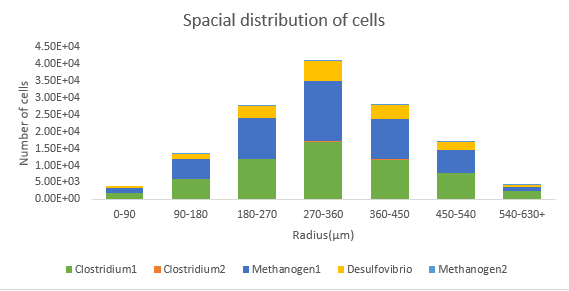
\includegraphics[width=1.0\textwidth]{images/spacial1.PNG}
\caption{Spacial distribution of cells across the granule.}
\label{fig:spacial1}
\end{figure}
\begin{figure}[htbp]
\centering
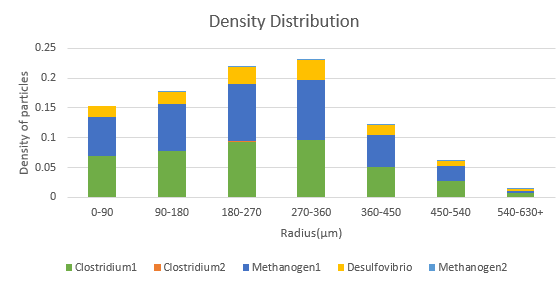
\includegraphics[width=1.0\textwidth]{images/spacial2.PNG}
\caption{Density of cells across the granule.}
\label{fig:spacial2}
\end{figure}



\subsection{Quantitative analysis of species biomass of the granule (Java)}

To determine the variation in biomass of the granule along with the species, we created a Java script which iterates over the files in Agent sum folder to record the amount of biomass present in each iteration for every species type. We wrote this data in a separate csv file and generated biomass vs time graphs using excel as shown in fig:\ref{fig:speciesgraph}

\begin{figure}[htbp]
\centering
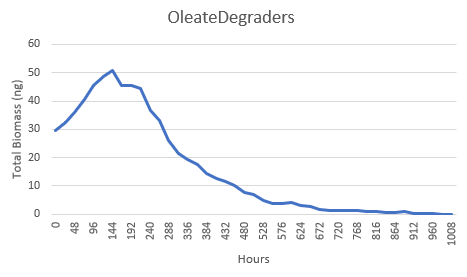
\includegraphics[width=1.0\textwidth]{images/speciesgraph.PNG}
\caption{Species biomass variation over time. }
\label{fig:speciesgraph}
\end{figure}

\subsection{Determining maximum solute concentration of each solute in every iteration among all the grid locations(Java)}

To compare the amount of solutes present at the end in various simulations(table:\ref{fig:maxsolutes}), we designed a Java script which iterates through every file in solute concentration directory to calculate and store the maximum value of each solute in a separate list.Once we have a list of all maximum concentrations for a particular species, we iterate over it to find the maximum value among them and use this value as the upper limit in MATLAB heatmap images to get uniform scaling in images. 

\begin{table}[]
\centering
\caption{Table containing maximum values of each solute for every simulation}
\label{maxsolutes}
\begin{tabular}{|l|l|l|l|l|l|l|}
\hline
\textbf{Solute}     & \textbf{Part 1} & \textbf{Part 2.1} & \textbf{Part 2.2} & \textbf{Part3.1.1} & \textbf{Part 2.3} & \textbf{Part 2.4} \\ \hline
\textbf{Cellobiose} & 2.5             & 0                 & 1                 & 2.5                & 2.5               & 2.5               \\ \hline
\textbf{Acetate}    & 0.827316476     & 0.620958594       & 0.186192785       & 0.026855469        & 0.017537938       & 0.159550879       \\ \hline
\textbf{Methane}    & 0.1883077       & 0.143837291       & 0.117415217       & 0.005836998        & 0.014162907       & 0.128956976       \\ \hline
\textbf{Lactate}    & 0.0122888       & 0.011243562       & 0.005570223       & 8.55E-04           & 9.44E-04          & 0.005545308       \\ \hline
\textbf{Ethanol}    & 0.001658617     & 0.000130947       & 0.000340241       & 3.25E-02           & 0.02994316        & 7.23E-04          \\ \hline
\textbf{Hydrogen}   & 0.018430389     & 0.018006731       & 0.00906213        & 0                  & 0.00106765        & 0.00926874        \\ \hline
\textbf{Oleate}     & 0               & 2.5               & 2.099757379       & 0                  & 0                 & 0                 \\ \hline
\end{tabular}
\end{table}


\subsection{Snapshots for spatial distribution of all the iterations to generate videos(Python)}

The spatial distribution scripts written in Java produced one file per iteration which consists of spatial distribution data of all species types.These files were used as inputs in a separate python script to generate spacial distribution line graphs for each iteration as shown in fig:\ref{fig:spatial3} . All the images for a single simulation were combined together to form a video demonstrating how the number of cells of each species type varies over the time across the granule.


\begin{figure}[htbp]
\centering
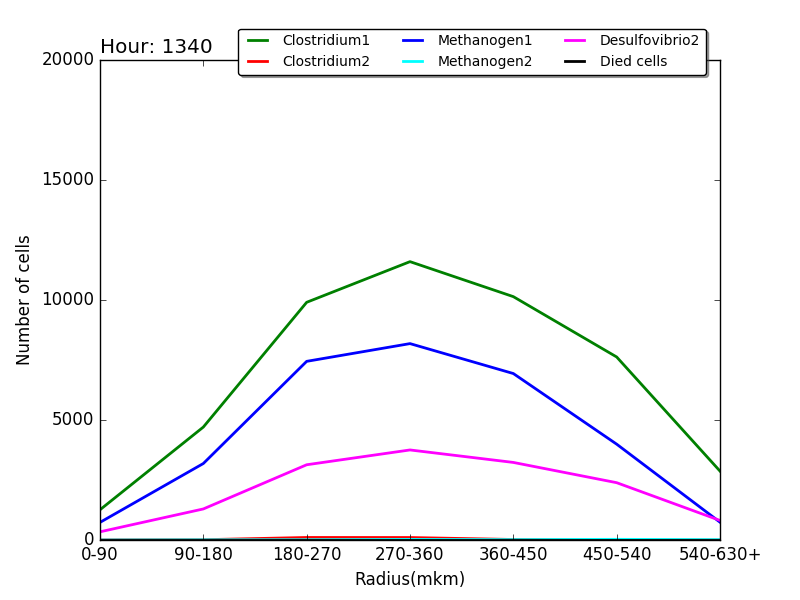
\includegraphics[width=1.0\textwidth]{images/spatial3.png}
\caption{Line graph for spatial distribution of species cells.}
\label{fig:spatial3}
\end{figure}

\chapter{DISCUSSION AND CONCLUSIONS}

The granule, which was initially grown and formed on the
cellulose as the main substrate, loses its mass and undergoes complete structure
changes, once placed into the new environment with oleate as the main substrate.
Biomass is initially drastically decreased, when the substrate is swapped. Once the
substrate is changed from cellulose to oleate, a different, two-species morphology of
the granule is established. New two-species granule begins to increase the total
biomass and diameter, but there are inclusions of the dead zones. The dead zones
are the microbes that were biochemically active previously, on cellulose, but were
forced to die, when the substrate was switched to the oleate.


    
    % Endmatter
    % For BibTeX references: specify a .bib file and a style.
    % The style used here is for IEEE transactions formatting:
    \references{IEEEabrv,sample}{IEEEtran}
    % The style used here is for AIAA formatting:
%    \references{IEEEabrv,sample}{aiaa}
    
    %
%  Example Appendix pages.
%  Modified to use new usu-thesis-mk2 appendix facilities.
%
%  Time-stamp: "[appendix.tex] last modified by Scott Budge (scott) on 2011-08-08 (Monday, 8 August 2011) at 15:46:06 on goga"
%
%  Info: $Id$   USU
%  Revision: $Rev$
% $LastChangedDate$
% $LastChangedBy$
%
%
% For a single appendix, use \makeappendix, and place the 
% body of the appendix after it

%\makeappendix

% < single appendix body here >

% For multiple appendices, use \makeappendices, and create each appendix
% using \appendix{}
% For sub-appendices use \appendixsection{} and \appendixsubsection{}

\makeappendices
\appendix{Input xml and result analysis code}
\label{chap:appendix}


\appendixsection{Description}

This xml document function as the definition of the model and as the input to the
simulation framework.


\label{sec:edge-def}

\appendixsection{Protocol file to generate the complex granule on cellobiose}

    \lstset{
    language=xml,
    tabsize=3,
    %frame=lines,
    caption=Input xml,
    label=code:sample,
    frame=shadowbox,
    rulesepcolor=\color{gray},
    xleftmargin=20pt,
    framexleftmargin=15pt,
    keywordstyle=\color{blue}\bf,
    commentstyle=\color{OliveGreen},
    stringstyle=\color{red},
    numbers=left,
    numberstyle=\tiny,
    numbersep=5pt,
    breaklines=true,
    showstringspaces=false,
    basicstyle=\footnotesize,
    emph={food,name,price},emphstyle={\color{magenta}}}
    \lstinputlisting{new2.xml}
    
    \appendixsection{Result analysis code to generate spatial distribution data}
    \lstset{frame=tb,
  language=Java,
  aboveskip=3mm,
  belowskip=3mm,
  showstringspaces=false,
  columns=flexible,
  caption=Species biomass calculator,
  basicstyle={\small\ttfamily},
  numbers=none,
  numberstyle=\tiny\color{gray},
  keywordstyle=\color{blue},
  commentstyle=\color{black},
  stringstyle=\color{red},
  breaklines=true,
  breakatwhitespace=true,
  tabsize=3
}
\lstinputlisting{BiomassGrowthAnalysis_Amitesh.java}

\appendixsection{Line graph generator for spatial distribution analysis}
    \lstset{frame=tb,
  language=Python,
  aboveskip=3mm,
  belowskip=3mm,
  showstringspaces=false,
  columns=flexible,
  caption=Python script to generate line graphs and save them as images,
  basicstyle={\small\ttfamily},
  numbers=none,
  numberstyle=\tiny\color{gray},
  keywordstyle=\color{blue},
  commentstyle=\color{black},
  stringstyle=\color{red},
  breaklines=true,
  breakatwhitespace=true,
  tabsize=3
}
\lstinputlisting{graphGenerator.py}
    
    
    
    



    %
% This is an example of a vita page.  
% Format is not tightly specified. This example comes from Lili Ma.
%
%  Time-stamp: "[vita.tex] last modified by Scott Budge (scott) on 2012-07-16 (Monday, 16 July 2012) at 11:18:06 on goga"
%
%  Info: $Id$   USU
%  Revision: $Rev$
% $LastChangedDate$
% $LastChangedBy$
%


    %}}}
\end{document}
